\begin{blocksection}
\question
Consider the 4-bit adder shown below. It takes:
\begin{itemize}
  \item a carry in (cin)
  \item two 4-bit inputs:
  \begin{itemize}
      \item a with bits \lstinline$a0, a1, a2, a3$
      \item b with bits \lstinline$b0, b1, b2, b3$
  \end{itemize}
\end{itemize}
And it outputs:
\begin{itemize}
  \item a carry out (cout)
  \item one 4-bit input: s with bits \lstinline$s0, s1, s2, s3$
\end{itemize}

Assume each adder has a delay of 10ns, and any registers have a clk-to-q, hold time, and setup time of 5ns. Assume the inputs are driven by registers, and outputs are registers as well.

Assume each adder has a delay of 10ns, and any registers have a clk-to-q, hold time, and setup time of 5ns. Assume the inputs are driven by registers, and outputs are registers as well.

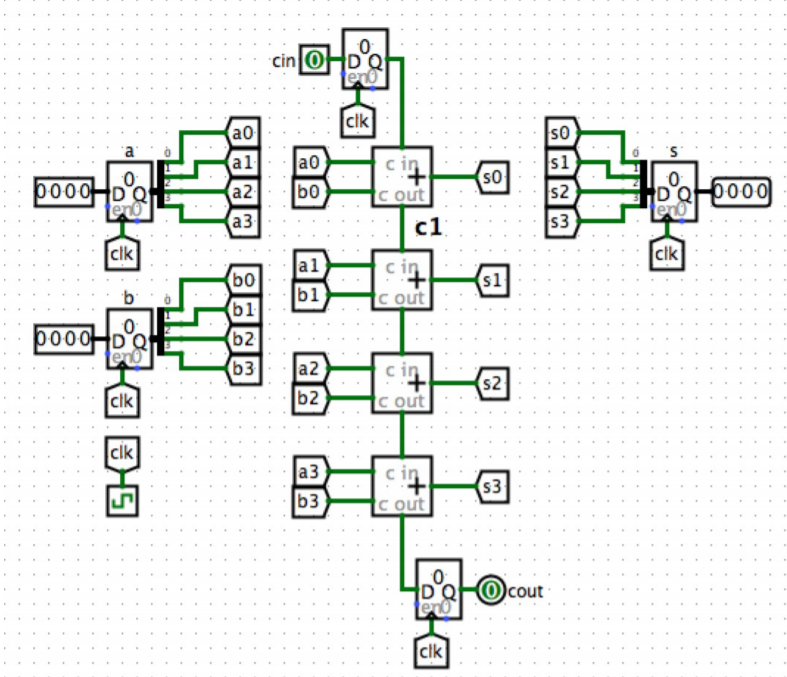
\includegraphics[width=0.8\textwidth]{midterm2/adder}

\end{blocksection}